% This is text associated with the open textbook "Open Electromagnetics"
% See immediately below for author, date
% This work is licensed under the Creative Commons Attribution-ShareAlike 4.0 International License. (CC BY-SA 4.0) 
% To view a copy of the license, visit http://creativecommons.org/licenses/by-sa/4.0/

%ORB TITLE Wave Propagation on a TEM Transmission Line
%ORB AUTHOR 0        # S.W. Ellingson, Virginia Tech (ellingson@vt.edu)
%ORB DATE 20180810   # yyyymmdd
%ORB ABSTRACT Solution of wave equation for TEM transmission line (current, potential); wavelength; phase velocity 

\label{m0080_Wave_Propagation_on_a_Transmission_Line} % <-- Must match name of this file and module directory name.  Don't mess with this!

In Section~\ref{m0027_Wave_Equations_for_a_Transmission_Line}, it is shown that expressions for the phasor representations of the potential and current along a transmission line are
%
\begin{equation}
\widetilde{V}(z) = V_0^+ e^{-\gamma z} + V_0^- e^{+\gamma z}
\label{m0080_eV}
\end{equation}
%
\begin{equation}
\widetilde{I}(z) = I_0^+ e^{-\gamma z} + I_0^- e^{+\gamma z}
\label{m0080_eI}
\end{equation}
%
where $\gamma$ is the propagation constant and it assumed that the transmission line is aligned along the $z$ axis.
In this section, we demonstrate that these expressions represent sinusoidal waves, and point out some important features.
Before attempting this section, the reader should be familiar with the contents of Sections~\ref{m0029_Lumped-Element_Model}, \ref{m0027_Wave_Equations_for_a_Transmission_Line}, and \ref{m0052_Characteristic_Impedance}.
A refresher on fundamental wave concepts (Section~\ref{m0074_Fundamentals_of_Waves}) may also be helpful.

We first define real-valued quantities $\alpha$ and $\beta$ to be the real and imaginary components of $\gamma$; i.e.,
%
\begin{equation}
\alpha \triangleq \mbox{Re}\left\{\gamma\right\}
\end{equation}
%
\begin{equation}
\beta \triangleq \mbox{Im}\left\{\gamma\right\}
\end{equation}
%
and subsequently
%
\begin{equation}
\gamma = \alpha + j\beta
\end{equation}
%
Then we observe
%
\begin{equation}
e^{\pm\gamma z} = e^{\pm\left(\alpha+j\beta\right)z} = e^{\pm\alpha z}~e^{\pm j\beta z}
\end{equation}
% 
It may be easier to interpret this expression by reverting to the time domain:
%
\begin{equation}
\mbox{Re}\left\{e^{\pm\gamma z}e^{j\omega t} \right\} = e^{\pm\alpha z}\cos\left(\omega t \pm \beta z\right)
\end{equation}
%
Thus, 
$e^{-\gamma z}$ represents a damped sinusoidal wave traveling in the $+z$ direction, and 
$e^{+\gamma z}$ represents a damped sinusoidal wave traveling in the $-z$ direction.
   
Let's define $\widetilde{V}^+(z)$ and $\widetilde{I}^+(z)$ to be the potential and current associated with a wave propagating in the $+z$ direction.  Then:
%
\begin{equation}
\widetilde{V}^+(z) \triangleq V_0^+ e^{-\gamma z} 
\end{equation}
%
or equivalently in the time domain:
%
\begin{flalign}
v^+(z,t) &= \mbox{Re}\left\{ \widetilde{V}^+(z) ~ e^{j\omega t} \right\} \nonumber \\
         &= \mbox{Re}\left\{ V_0^+ e^{-\gamma z}  e^{j\omega t} \right\} \nonumber \\
         &= \left|V_0^+\right| e^{-\alpha z}\cos\left(\omega t - \beta z +\psi\right) 
\end{flalign}
%
where $\psi$ is the phase of $V_0^+$.
Figure~\ref{m0080_fVwave} shows $v^+(z,t)$. 
From fundamental wave theory we recognize 
%
%ORB HIGHLIGHT
\begin{mdframed}[backgroundcolor=yellow!20,nobreak=true] 
$\beta\triangleq\mbox{Im}\left\{\gamma\right\}$ (rad/m) is the \emph{phase propagation constant}, 
\index{propagation constant!phase}
which is the rate at which phase changes as a function of distance.  
\end{mdframed}
%
Subsequently the wavelength in the line is
%
\begin{equation}
\boxed{ \lambda = \frac{2\pi}{\beta} }
\end{equation}
%
\begin{figure}
\begin{center}
\pdftooltip{{  % note double braces
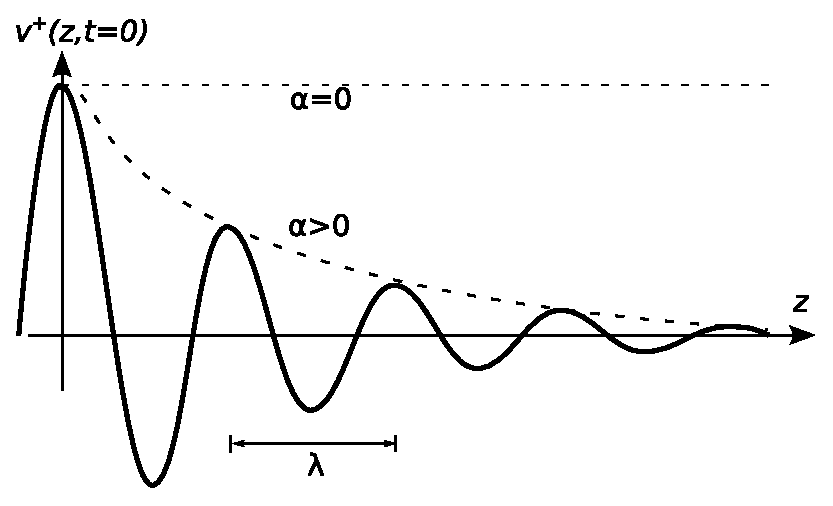
\includegraphics[width=\columnwidth]{modules/m0080_fVwave.eps}
}}{A graph depicting a wave traveling across the z-axis with 5 peaks. The first wave peak intersects the y-axis and is labeled v superscript + (z,t=0). At the top of the first peak, a dotted line extends perpendicularly to the right labeled alpha=0. Also at the top of the first peak, a dotted line curves downward with decreasing slope and is labeled alpha>0. As the wave oscillates to the right along the z-axis, the peaks decrease in height. Between the second and third peaks, a line underneath the graph shows the wavelength lambda.}
\end{center} 
\caption{\label{m0080_fVwave}The potential $v^+(z,t)$ of the wave traveling in the $+z$ direction at $t=0$ for $\psi=0$.}
\end{figure}

Also we recognize:
%ORB HIGHLIGHT
\begin{mdframed}[backgroundcolor=yellow!20,nobreak=true] 
$\alpha\triangleq\mbox{Re}\left\{\gamma\right\}$ (1/m) is the \emph{attenuation constant}, 
\index{propagation constant!attenuation}
\index{attenuation constant|see {propagation constant}}
which is the rate at which magnitude diminishes as a function of distance. 
\end{mdframed}

Sometimes the units of $\alpha$ are indicated as ``Np/m'' (``nepers'' per meter), where the term ``neper'' 
\index{neper}
is used to indicate the units of the otherwise unitless real-valued exponent of the constant $e$.

Note that $\alpha=0$ for a wave that does not diminish in magnitude with increasing distance, in which case the transmission line is said to be \emph{lossless}.
\index{transmission line!lossless}
If $\alpha>0$ then the line is said to be \emph{lossy} (or possibly ``low loss'' if the loss can be neglected), 
\index{transmission line!low loss}
and in this case the rate at which the magnitude decreases with distance increases with $\alpha$.  

Next let us consider the speed of the wave.
To answer this question, we need to be a bit more specific about what we mean by ``speed.''
At the moment, we mean phase velocity; 
that is, the speed at which a point of constant phase seems to move through space.
In other words, what distance $\Delta z$ does a point of constant phase traverse in time $\Delta t$?
To answer this question, we first note that the phase of $v^+(z,t)$ can be written generally as 
%
\begin{equation}
\omega t - \beta z + \phi
\nonumber
\end{equation}
%
where $\phi$ is some constant.  
Similarly, the phase at some time $\Delta t$ later and some point $\Delta z$ further along can be written as 
%
\begin{equation}
\omega \left( t +\Delta t \right) - \beta \left( z +\Delta z \right) + \phi
\nonumber
\end{equation}
The phase velocity $v_p$ is $\Delta z/\Delta t$ when these two phases are equal; i.e., when
%
\begin{equation}
\omega t - \beta z + \phi = \omega \left( t +\Delta t \right) - \beta \left( z +\Delta z \right) + \phi
\nonumber
\end{equation}   
%
Solving for $v_p=\Delta z/\Delta t$, we obtain:
%
\begin{equation}
\boxed{ v_p = \frac{\omega}{\beta} }
\end{equation}
%
Having previously noted that $\beta = 2\pi/\lambda$, the above expression also yields the expected result
%
\begin{equation}
\boxed{
v_p = \lambda f
}
\end{equation}
%
%ORB HIGHLIGHT
\begin{mdframed}[backgroundcolor=yellow!20,nobreak=true] 
The phase velocity 
\index{phase velocity}
$v_p = \omega/\beta = \lambda f$ is the speed at which a point of constant phase travels along the line.
\end{mdframed}

Returning now to consider the current associated with the wave traveling in the $+z$ direction:
%
\begin{equation}
\widetilde{I}^+(z) = I_0^+ e^{-\gamma z} 
\end{equation}
%
We can rewrite this expression in terms of the characteristic impedance 
\index{characteristic impedance}
$Z_0$, as follows:
%
\begin{equation}
\widetilde{I}^+(z) = \frac{V_0^+}{Z_0} e^{-\gamma z}
\end{equation}
%
Similarly, we find that the current $\widetilde{I}^-(z)$ associated with $\widetilde{V}^-(z)$ for the wave traveling in the $-z$ direction is
%
\begin{equation}
\widetilde{I}^-(z) = \frac{-V_0^-}{Z_0} e^{-\gamma z}
\end{equation}
%
The negative sign appearing in the above expression emerges as a result of the sign conventions used for potential and current in the derivation of the telegrapher's equations (Section~\ref{m0079_Telegraphers_Equations}).
The physical significance of this change of sign is that wherever the potential of the wave traveling in the $-z$ direction is positive, then the current at the same point is flowing in the $-z$ direction. 

It is frequently necessary to consider the possibility that waves travel in both directions simultaneously. 
A very important case where this arises is when there is reflection from a discontinuity of some kind; e.g., from a termination which is not perfectly impedance-matched.
In this case, the total potential $\widetilde{V}(z)$ and total current $\widetilde{I}(z)$ can be expressed as the general solution to the wave equation; i.e., as the sum of the ``incident'' ($+z$-traveling) wave and the reflected ($-z$-traveling) waves:
%
\begin{equation}
\widetilde{V}(z) = \widetilde{V}^+(z) + \widetilde{V}^-(z)
\end{equation}
%
\begin{equation}
\widetilde{I}(z) = \widetilde{I}^+(z) + \widetilde{I}^-(z)
\end{equation}
%
The existence of waves propagating simultaneously in both directions gives rise to a phenomenon known as a \emph{standing wave}. 
\index{waves!standing|see{standing wave}}
\index{standing wave}
Standing waves and the calculation of the coefficients $V_0^{-}$ and $I_0^{-}$ due to reflection are addressed in Sections~\ref{m0086_Standing_Waves} and \ref{m0084_Voltage_Reflection_Coefficient} respectively.

